We can represent the systems of equations in Equation \ref{eq:galerkin_form} and Equation \ref{eq:jacobian_form} as a series of computational kernels, which may be fused in certain implementations.
This streamlined representation is used by \href{https://www.github.com/CEED/libCEED}{libCEED} \cite{libceed-user-manual} to provide performance portable implementations.
In Chapter \ref{ch:LocalFourierAnalysis}, we use this representation to develop LFA of high-order finite element operators and preconditioning methods.

The action of an arbitrary second-order finite element operator can be represented as
\begin{equation}
{\color{burgundy}\mathbf{A}} = \mathbf{P}^T \mathbf{G}^T {\color{blue(ncs)}\mathbf{B}}^T {\color{applegreen}\mathbf{D}} {\color{blue(ncs)}\mathbf{B}} \mathbf{G} \mathbf{P}
\label{eq:libceed_representation}
\end{equation}

where $\mathbf{P}$ represents the parallel communication portion of the global element restriction operator, $\mathbf{G}$ represents the device portion of the global element restriction operator, ${\color{blue(ncs)}\mathbf{B}}$ represents the basis action kernel that provides solution values and derivatives at the quadrature points, and ${\color{applegreen}\mathbf{D}}$ represents the pointwise representation of the weak form, given by $f_i$ or $f_{i, j}$ and the element quadrature weights and geometric factors.

\begin{figure}[ht!]
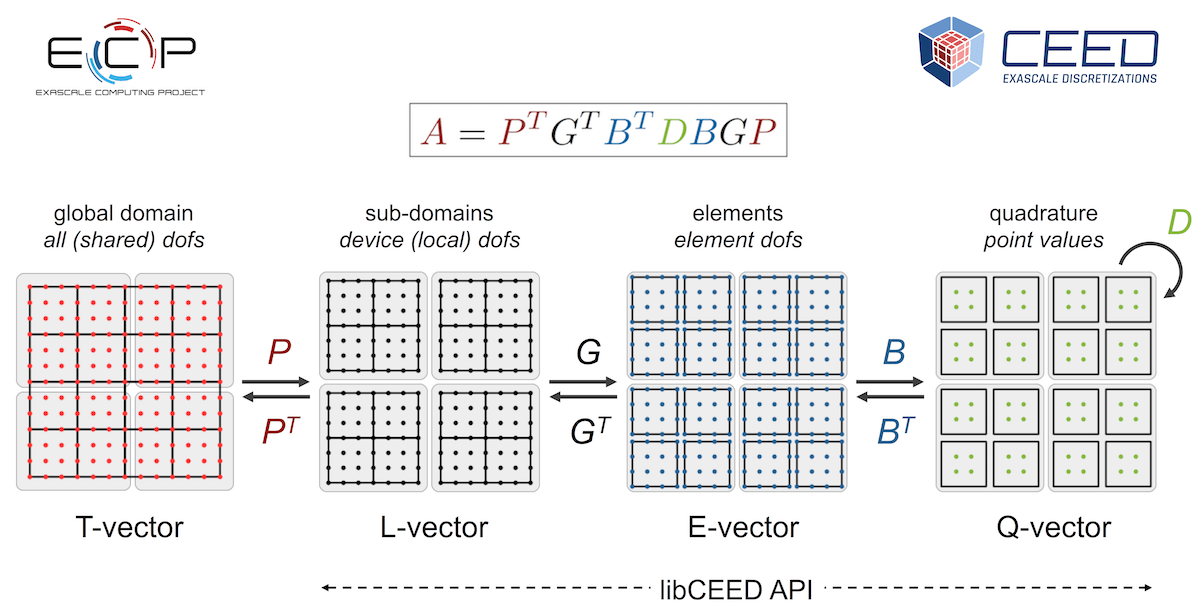
\includegraphics[width=.99\linewidth]{../img/libCEEDAPI}
\caption{\href{https://www.github.com/CEED/libCEED}{libCEED} API}
\label{fig:libceedapi}
\end{figure}

This representation is shown graphically in Figure \ref{fig:libceedapi}, where we can see the different spaces that each kernel operates upon.
This flexible kernel representations will be used in Chapter \ref{ch:LocalFourierAnalysis}, where we develop Local Fourier Analysis of finite element operators that can be represented in this fashion.
{\bf \color{burgundy}Burgundy} text will be used to represent operators that can be implemented in this matrix-free representation.
